\documentclass[11pt]{article}
\usepackage{geometry}                % See geometry.pdf to learn the layout options. There are lots.
\geometry{letterpaper}                   % ... or a4paper or a5paper or ... 
%\geometry{landscape}                % Activate for for rotated page geometry
%\usepackage[parfill]{parskip}    % Activate to begin paragraphs with an empty line rather than an indent
\usepackage{graphicx}
\usepackage{amssymb}
\usepackage{amsmath}
\usepackage{epstopdf}
\usepackage{hyperref}
\usepackage{natbib}
\DeclareGraphicsRule{.tif}{png}{.png}{`convert #1 `dirname #1`/`basename #1 .tif`.png}


\graphicspath{
{/Users/Andy/Cruises_Research/Chipod/}
}

\title{CTD-$\chi$pod Processing Guide}
\author{Andy Pickering}
%\date{}                                           % Activate to display a given date or no date


\begin{document}
\maketitle

\tableofcontents
\newpage


%~~~~~~~~~~~~~~~~~~~~~~~~~~~~~~~~~~~~~~
\section{Introduction}

This is a guide to processing data from CTD-$\chi$pods. $\chi$pods are self-contained instruments developed by the OSU Ocean Mixing Group to measure turbulence. They have a FP07 thermistor that measures temperature and temperature gradient, sampled at 100Hz. 

 
%~~~~~~~~~~~~~~~~~~~~~~~~~~~~~~~~~~~~~~
\section{Brief Outline of Major Processing Steps}

\begin{enumerate}
\item Find chipod data for each CTD cast
\item Align chipod data with CTD data
\item Calibrate chipod data
\item Apply chipod calc in 1 sec windows
\end{enumerate}
More details are given in the rest of the document.



%~~~~~~~~~~~~~~~~~~~~~~~~~~~~~~~~~~~~~~
\section{Software}
The processing is done with Matlab codes, which are maintained in a github repository: \newline
 \url{https://github.com/OceanMixingGroup/mixingsoftware}.\newline
  The CTD-$\chi$pod specific codes are in the folder \verb+/CTD_Chipod+. Codes for processing raw CTD data (.hex format) are contained in \verb+/ctd_processing+.



%~~~~~~~~~~~~~~~~~~~~~~~~~~~~~~~~~~~~~~
\section{Preferred Data Organziation}

\begin{itemize}
\item \verb+/Data/raw/Chipod/SNxxxx+ : Raw $\chi$pod data.
\item \verb+/Data/raw/CTD/+ : Raw CTD data (.hex,.XMLCON,.hdr).
\item \verb+/Data/proc/Chipod+ Processed $\chi$pod data
\item \verb+/Data/proc/CTD+ Processed CTD data. (/24Hz,/binned).
\end{itemize}


%~~~~~~~~~~~~~~~~~~~~~~~~~~~~~~~~~~~~~~
\section{CTD data}

CTD data needs to be obtained and processed before running the $\chi$pod processing.
Processing requires:
\begin{enumerate}
\item 24Hz data: used to determine the time offset between the CTD data and $\chi$pod data, by aligning (highpassed) dp/dt from the CTD with w estimated by integrating vertical chipod accelerations. 24Hz temperature is also used to calibrate the chipod temperature voltages and convert to physical units.
\item 1-m binned data: used to calibrate chi-pod T, and calculate dT/dz and $N^2$. 
\end{enumerate} 

I prefer to use codes in \verb+/mixingsoftware/ctd_processing/+ to process standard Seabird hex files into standard mat files to use in chi-pod processing. See \verb+Process_CTD_hex_Template.m+ for an example. The data can be processed using other methods, but must contain the specific fields required by the processing routines as listed below:

\subsection{24Hz CTD Data}

Required fields for 24Hz CTD data are:
\begin{itemize}
\item  dnum : datenum
\item t : temperature [C]
\item p : pressure [db]
\end{itemize}

\subsection{1-m Binned CTD Data}
Required fields for binned CTD data
\begin{itemize}
\item dnum : datenum
\item t : temperature [C]
\item p : pressure [db]
\item s : salinity
\item lat : Latitude 
\item lon : Longitude
\end{itemize}



%~~~~~~~~~~~~~~~~~~~~~~~~~~~~~~~~~~~~~~
\section{Processing steps}

\begin{enumerate}
\item Modify \verb+Load_chipod_paths_template.m+ . This specifies filepaths to raw data, as well as where output will be saved.
\item Modify \verb+Chipod_Deploy_Info_template.m+ with info for specific deployment. Much of the rest of the processing uses information from the above two files.
\item Plot the raw chi-pod data (\verb+Plot_Raw_Data_template+?). This will let you see quickly if any sensors or files are obviously bad. If there are bad files you can specify these in a \verb+Bad_File�+  list so they will not be loaded during processing (this is not necessary, but will reduce time loading bad files, and may prevent bad data from accidentally being used).  Figure \ref{x} shows an example of a normal-looking file. Figure \ref{xx} shows an example of file that looks bad.
\item  Modify \verb+MakeCasts_CTDchipod_Template.m+ for specific cruise. This script finds $\chi$pod data for each cast, aligns the data, calibrates the data, and saves a file with data for each cast.
\item  Run \verb+MakeCasts_CTDchipod+ for one good cast for each SN. Check time-offset / alignment; if not right, probably need to modify \verb+az_correction+ or switch AX and AZ. Figure \ref{x} shows an example of where AX and AZ are flipped.  * figures showing example of flipped ax etc*
\item  Once that is figured out, run \verb+MakeCasts_CTDchipod+ for all casts.
\item  Modify \verb+DoChiCalc_Template.m+ and run for all casts. This does the chi calculation for all the cast files made in \verb+MakeCasts_CTDchipod+.
\item Make summary plots


\end{enumerate}



%~~~~~~~~~~~~~~~~~~~~~~~~~~~~~~~~~~~~~~
\section{$\chi$pod Processing Parameters}

Variable parameters for the processing are specified in a `Params' structure.

\begin{itemize}
\item fmax : Maximum frequency to integrate temperature gradient spectrum to (default 20Hz).
\item gamma : Assumed mixing efficiency (default 0.2).
\item \verb+resp_corr+ : Option to apply frequency response correction.
\item fc : Cutoff frequency for response correction (if applied).
\item \verb+z_smooth+ : The distance [m] over which $N^2$ and $dT/dz$ are smoothed.
\end{itemize}



%~~~~~~~~~~~~~~~~~~~~~~~~~~~~~~~~~~~~~~
\section{Output File Formats}

\subsection{cast}
`Raw' $\chi$pod data for each cast, with fields:
\begin{itemize}
\item adsf
\end{itemize}
Ex. filename : \verb++

\subsection{cal}
Calibrated data for each cast. Up and down casts are saved in separate files.
\begin{itemize}
\item adsf
\end{itemize}
Ex. filename : \verb++

\subsection{avg}
Result of $\chi$pod calculations. Contains data points for each 1 sec window.
\begin{itemize}
\item adsf
\end{itemize}
Ex. filename : \verb++




%~~~~~~~~~~~~~~~~~~~~~~~~~~~~~~~~~~~~~~
\section{Post-processing Analysis}

\begin{itemize}
\item Plot $\chi$pod time-offsets. The time-offset should drift linearly with time, and may be reset during the cruise. Typically should be less than 20 sec (depends on how accurately time was set). In some cases, the time was set wrong (off by a day, wrong time zone etc.); in this case the processing script needs to be modified to correct this.
\item Compare different sensors and cast directions: The quality of data obtained depends heavily on the setup of the CTD and the $\chi$pod mounting. Typically the upward looking sensors on the upcasts are the cleanest data. 
\item Sensitivity to parameters: see details below.
\end{itemize}



%~~~~~~~~~~~~~~~~~~~~~~~~~~~~~~~~~~~~~~
\section{Sensitivity Analysis}







%~~~~~~~~~~~~~~~~~~~~~~~~~~~~~~~~~~~~~~
\section{Standard Plots made by processing}

\begin{itemize}
\item \verb+cast_001_RawChipodTS+ (Figure \ref{tsraw}).
\item \verb+cast_001_w_dTdtSpectraCheck+ (Figure \ref{speccheck}).
\item \verb+cast_001_w_TimeOffset+ (Figure \ref{align})
\item \verb+cast_001_w_TimeOffset_Zoom+ (Figure \ref{alignzoom})
\item \verb+cast_001_T_P_dTdz_fspd+ (Figure \ref{tscal})
\item \verb+cast_001_upcast_chi_SN600_T1_avg_chi_KT_dTdz+ (Figure \ref{avgsum})

\end{itemize}


\begin{figure}[s]
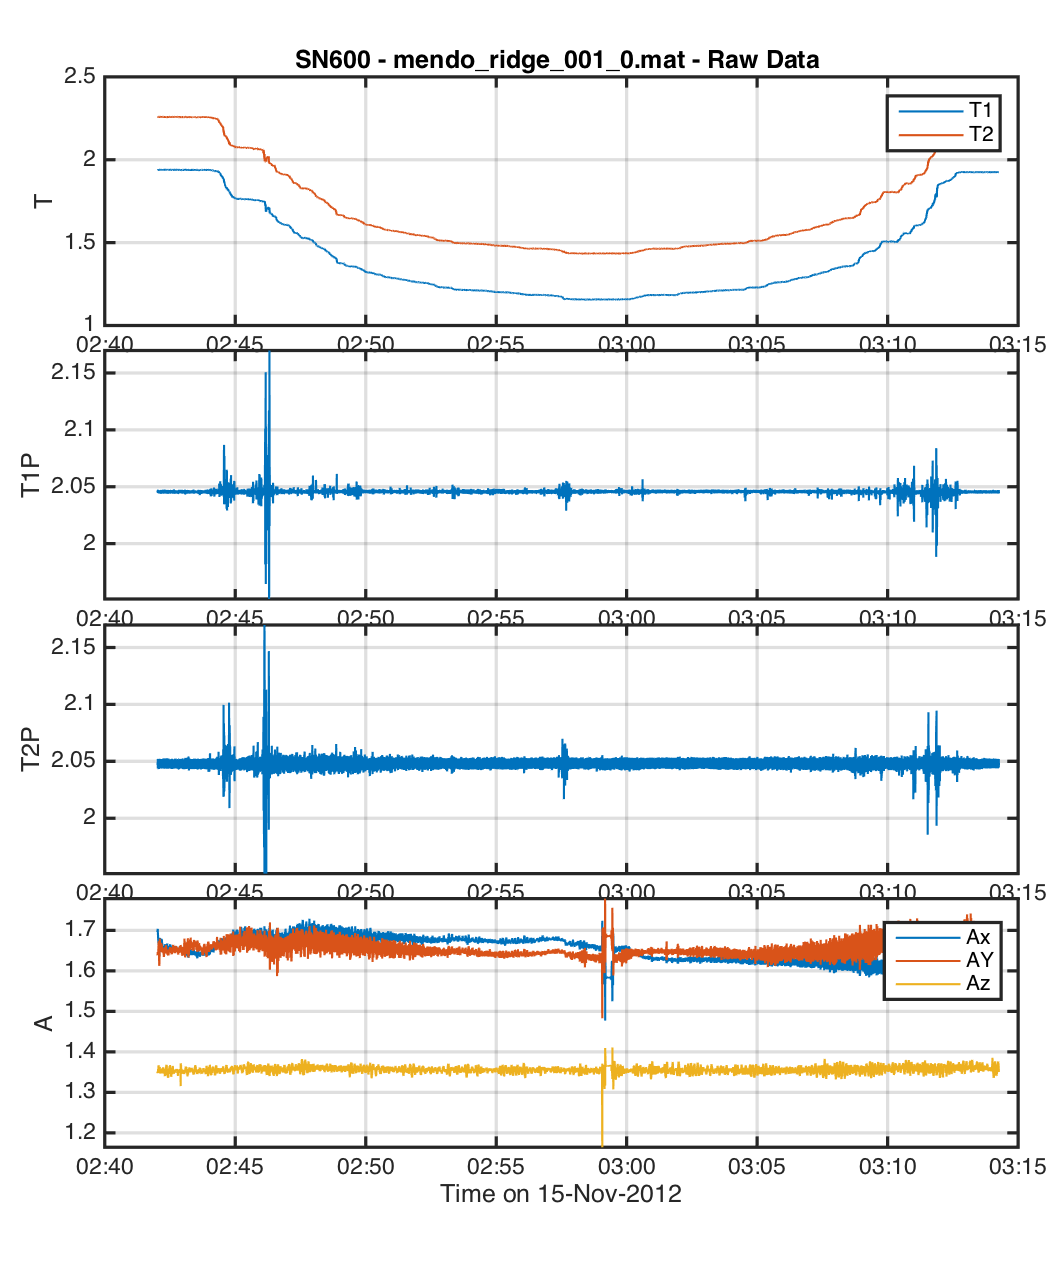
\includegraphics[scale=0.75]{cast_001_RawChipodTS.png}
\caption{Time-series of raw $\chi$pod data for one cast.}
\label{tsraw}
\end{figure}


\begin{figure}[s]
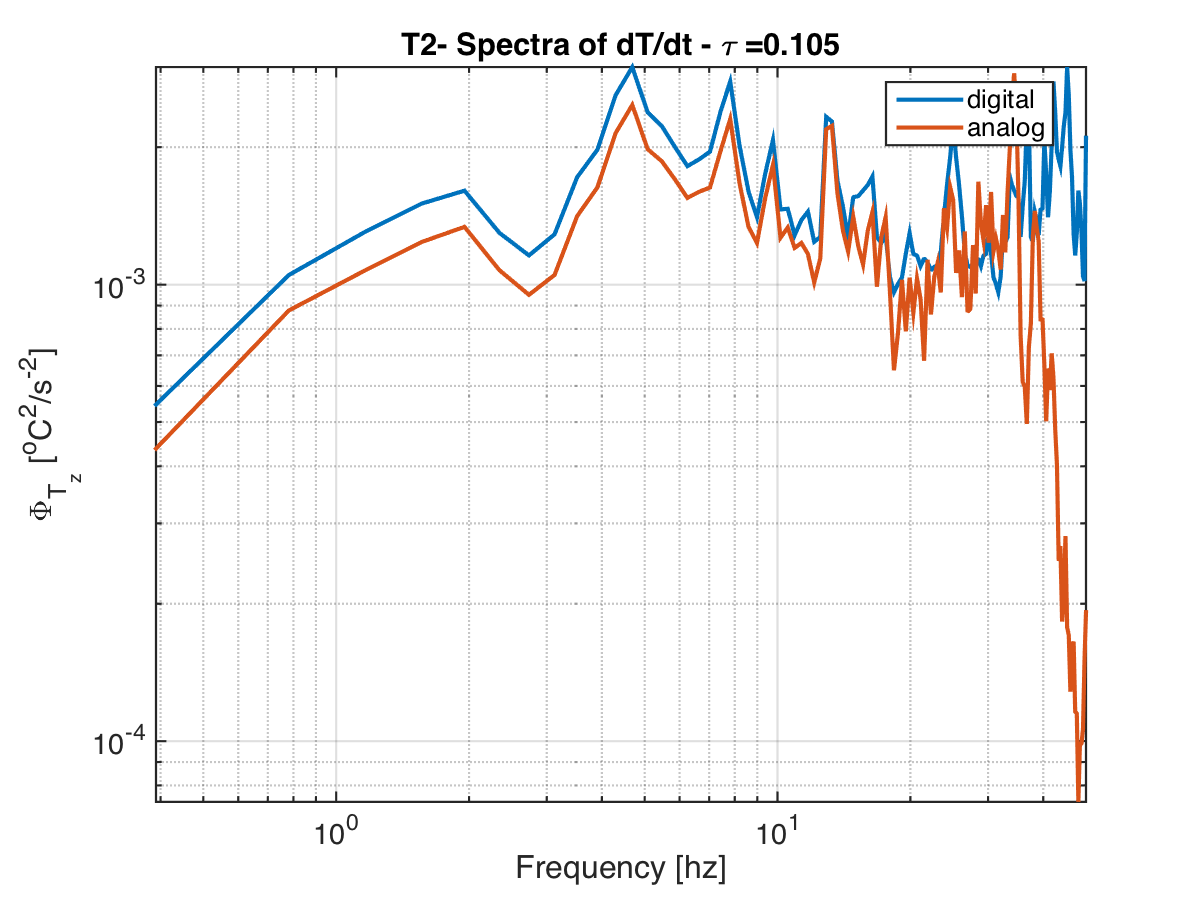
\includegraphics[scale=0.75]{cast_001_w_dTdtSpectraCheck.png}
\caption{dT/dt spectra for analog (TP) and digital derivatives. Spectra levels should match; if not time-constant may be wrong.}
\label{speccheck}
\end{figure}

\begin{figure}[s]
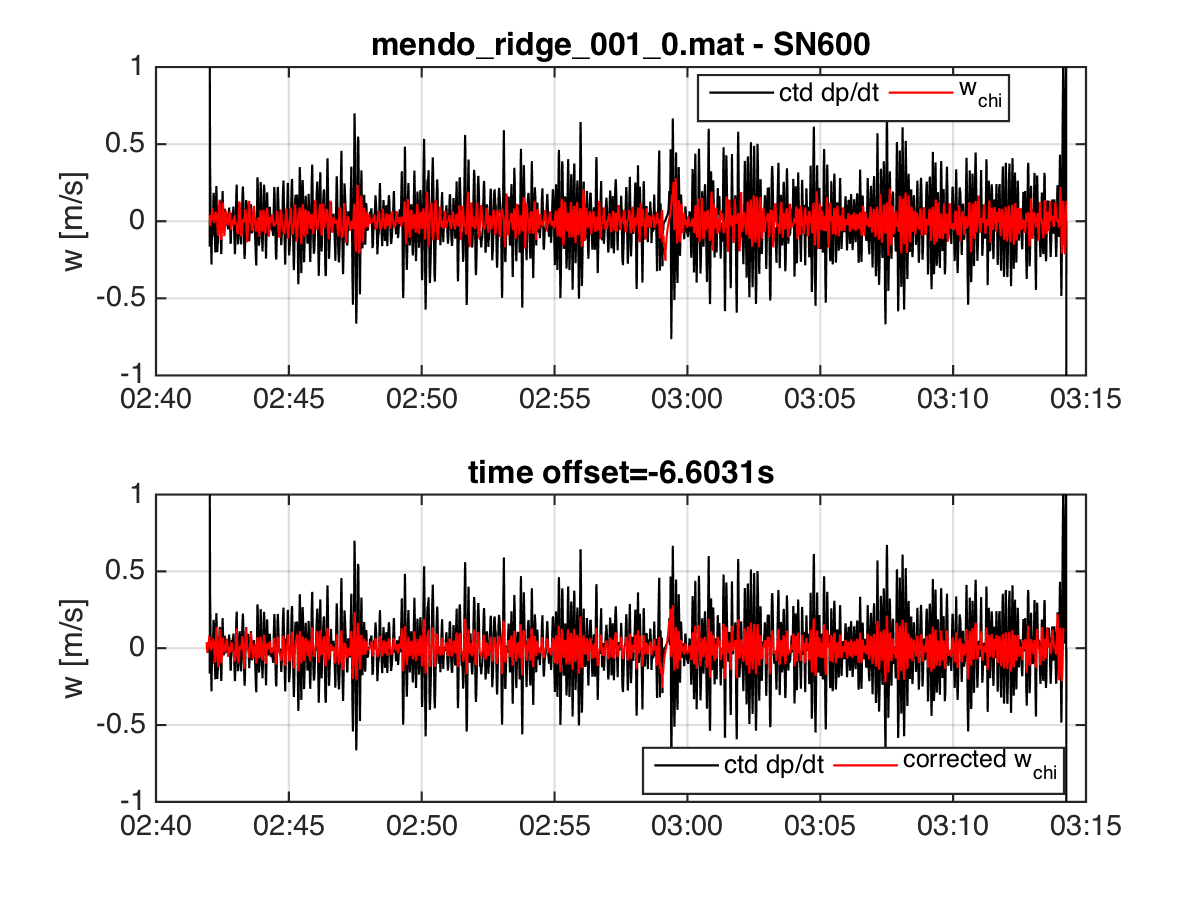
\includegraphics[scale=0.75]{cast_001_w_TimeOffset.png}
\caption{Time series of dp/dt CTD and chipod w. Top is original, bottom is after time-offset applied to chipod.}
\label{align}
\end{figure}

\begin{figure}[s]
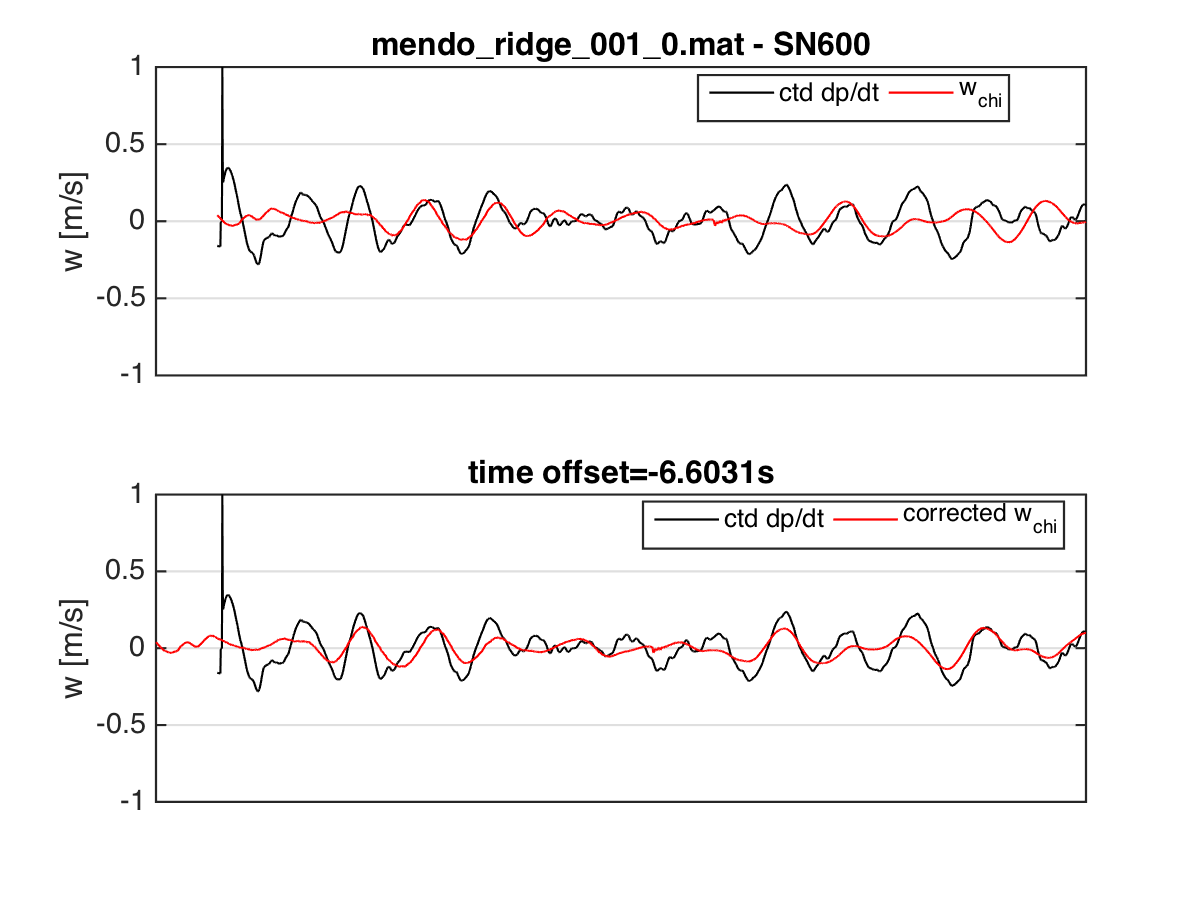
\includegraphics[scale=0.75]{cast_001_w_TimeOffset_Zoom.png}
\caption{Zoom-in of dp/dt and chipod w allowing one to check if time-offset is correct. Bottom panel should match.}
\label{alignzoom}
\end{figure}

\begin{figure}[s]
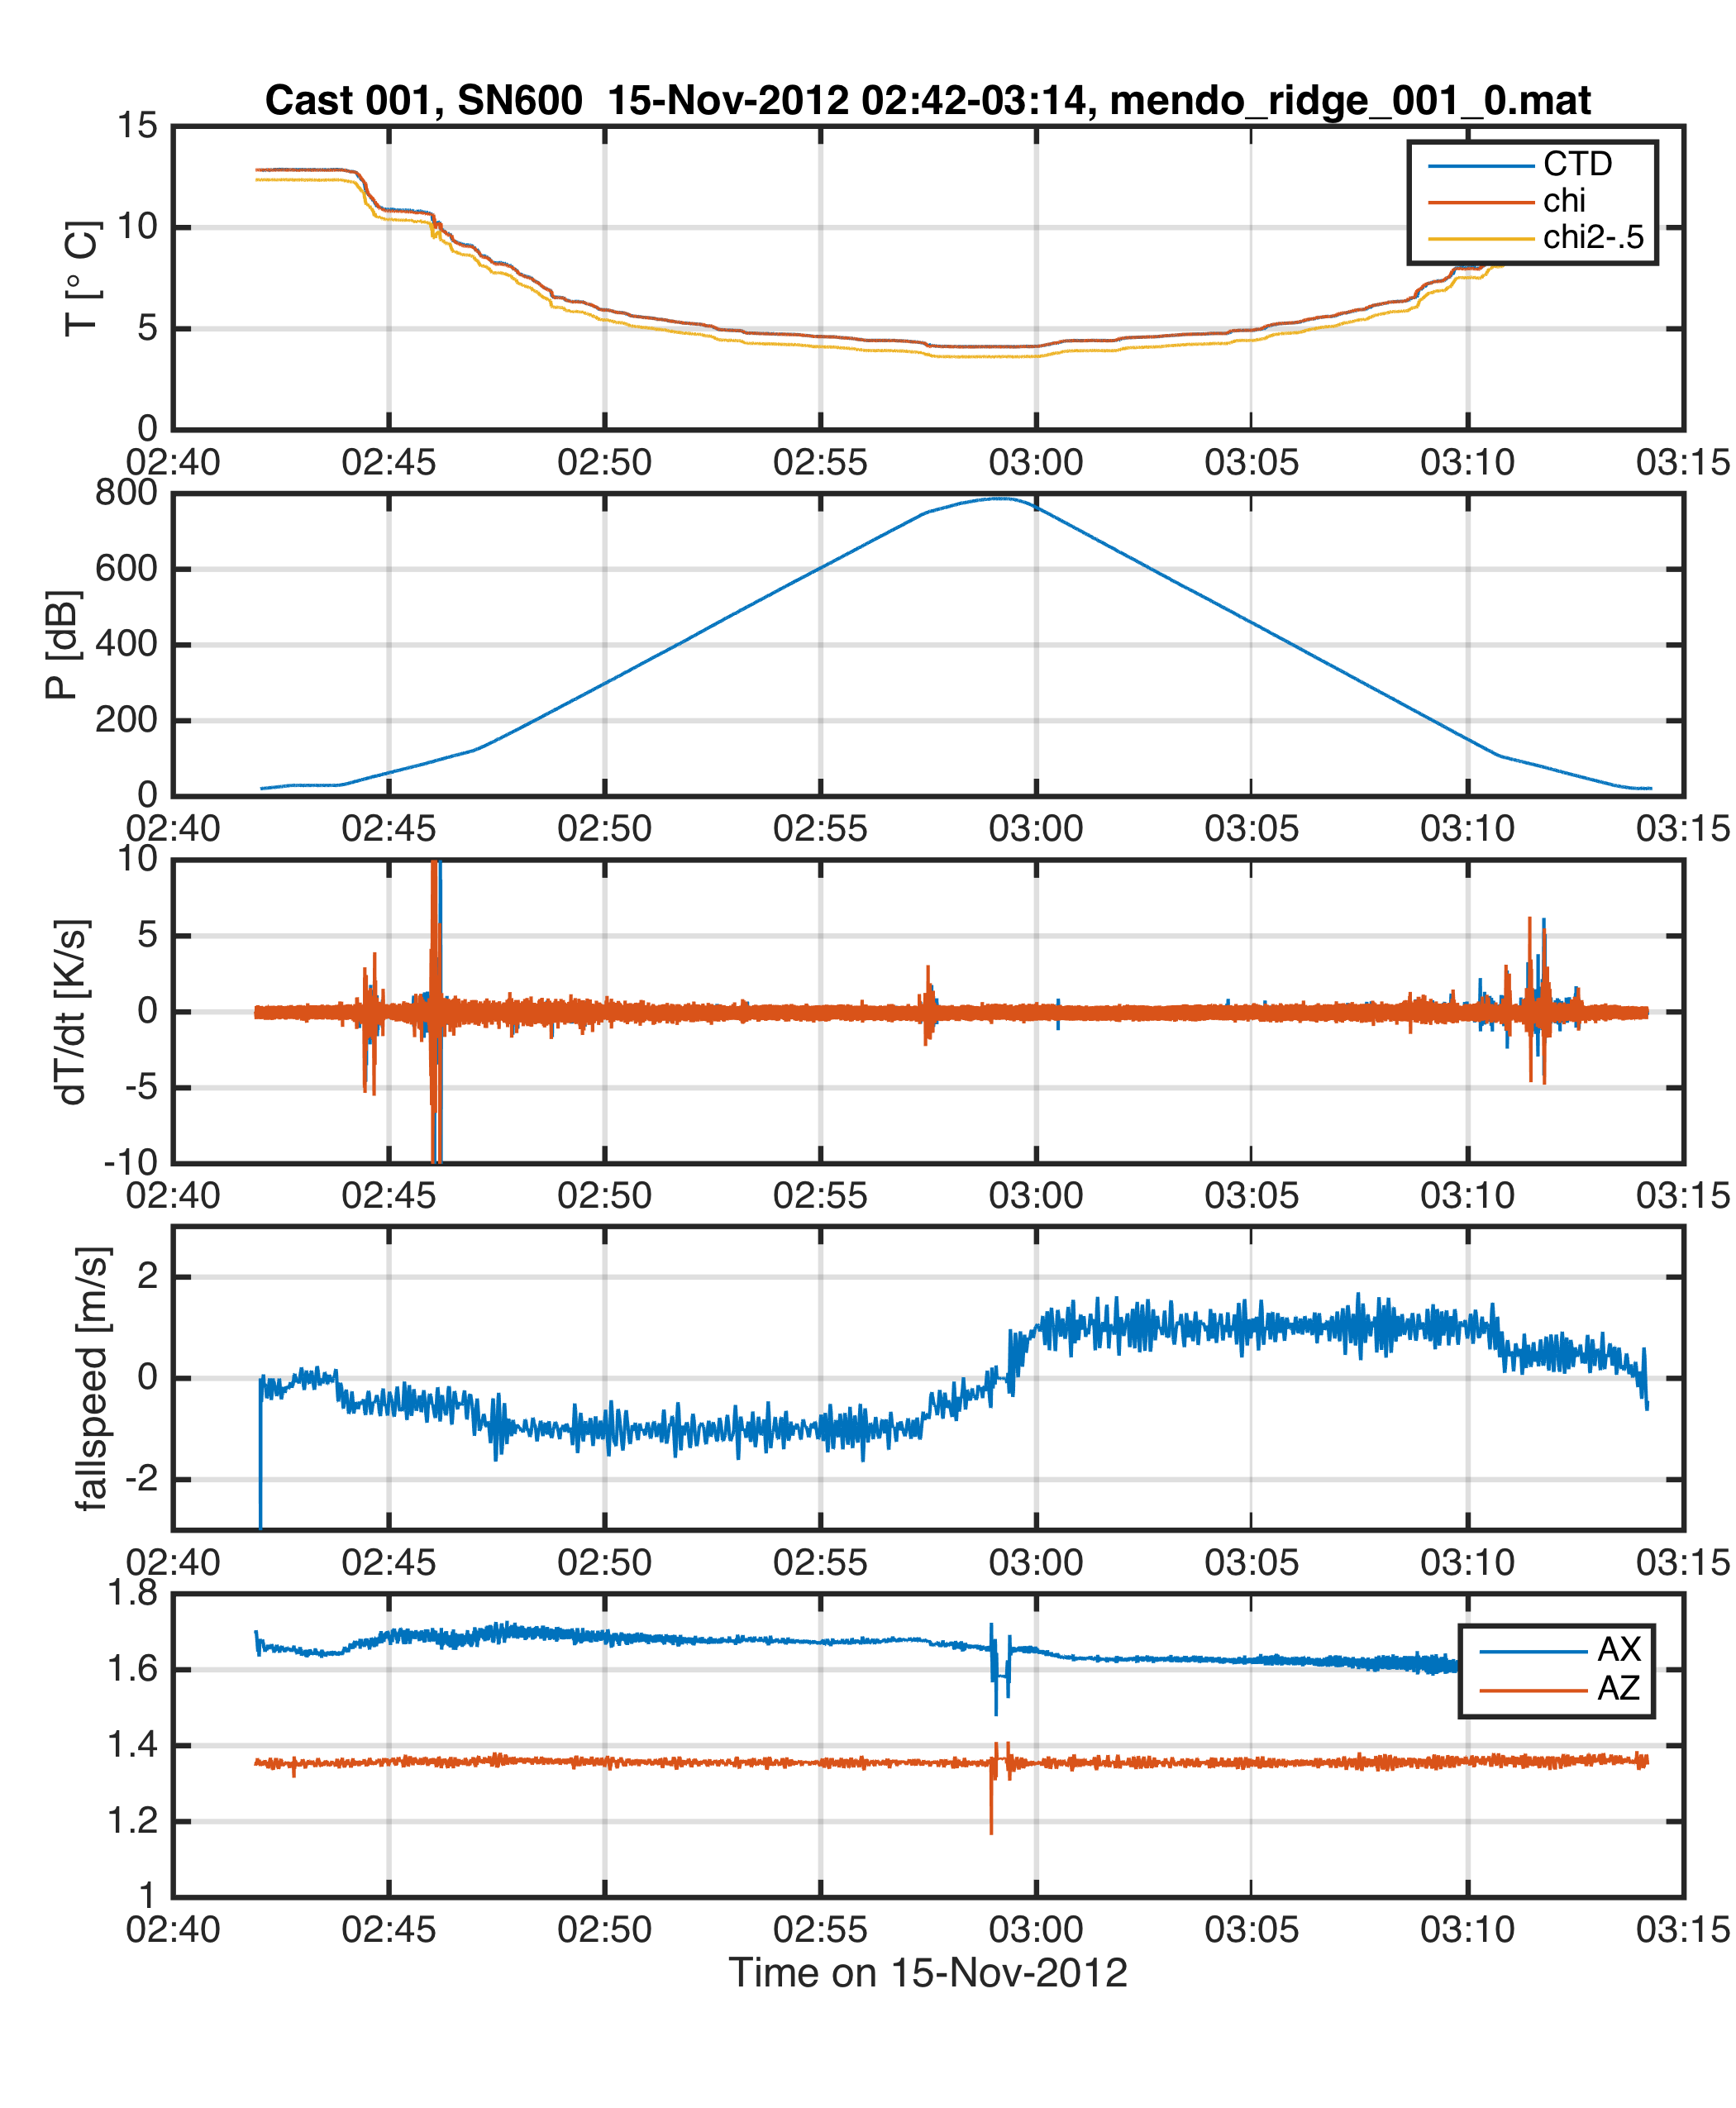
\includegraphics[scale=0.75]{cast_001_T_P_dTdz_fspd.png}
\caption{Time series of aligned and calibrated chipod data for one cast.}
\label{tscal}
\end{figure}


\begin{figure}[s]
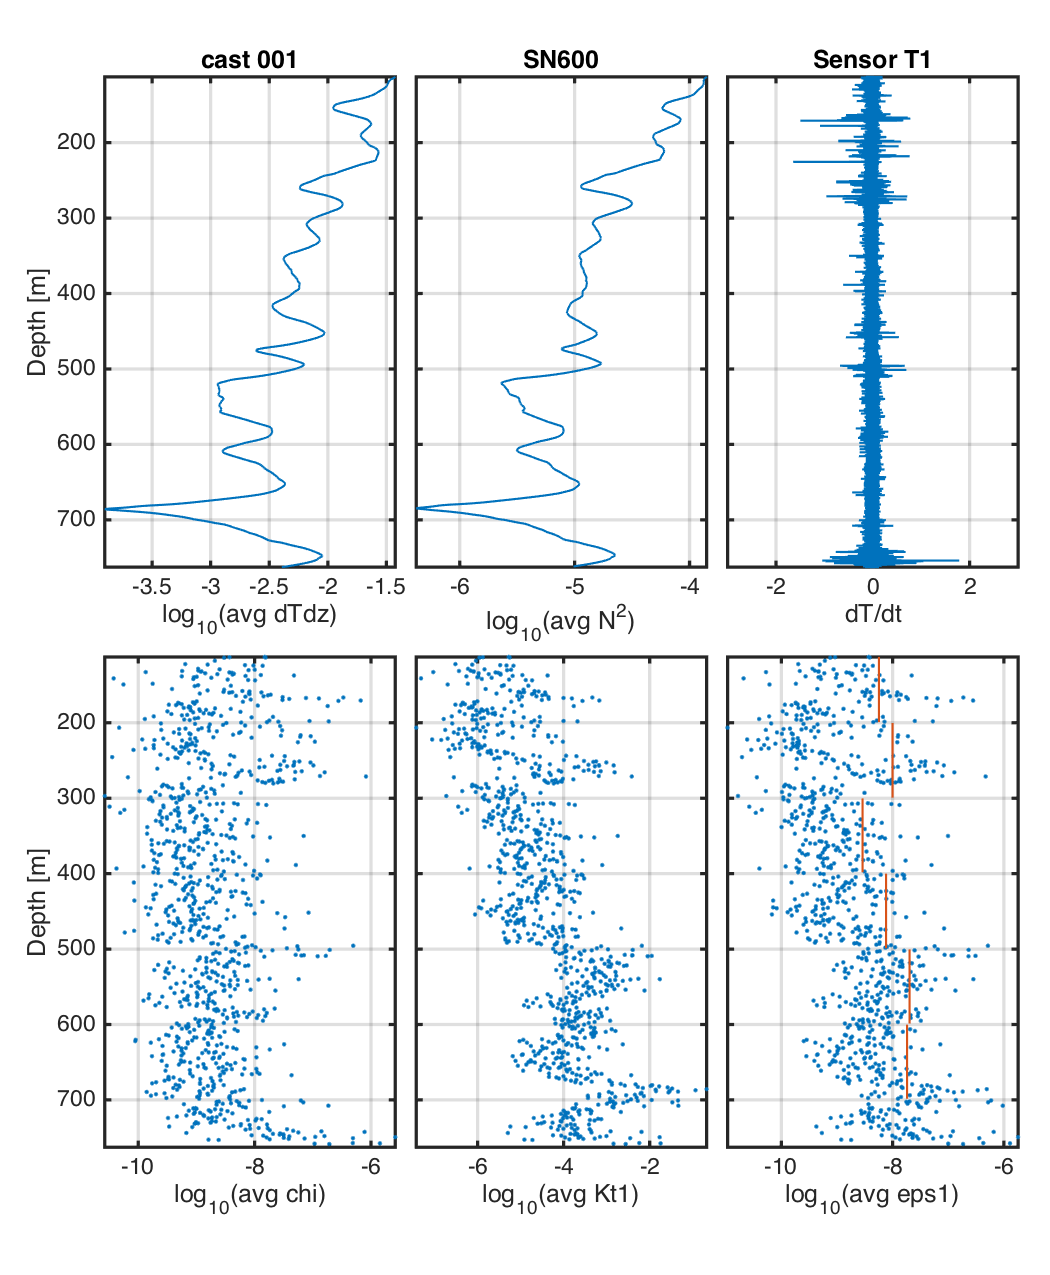
\includegraphics[scale=0.75]{cast_001_downcast_chi_SN600_T1_avg_chi_KT_dTdz.png}
\caption{Results of chipod calculation for one cast. Red lines in lower panel are 100m? binned averages.}
\label{avgsum}
\end{figure}



%~~~~~~~~~~~~~~~~~~~~~~~~~~~~~~~~~~~~~~
\section{m-files}

Processing files are kept in a GitHub repository \verb+/mixingsoftware/CTD_Chipod/+

\begin{itemize}
\item \verb+AlignChipodCTD+ : Align CTD and chipod data.
\item \verb+Compute_N2_dTdz_forChi+
\item \verb+get_chipod_chi+ : Main function that does chipod calculation.
\item \verb+load_chipod_data+
\item \verb+MakeCtdChiWindows+
\item \verb++
\end{itemize}



%\section{About}
%\begin{figure}[s]
%\includegraphics[scale=0.75]{XXXX_map.png}
%\caption{Map of CTD cast locations during cruise XXXX.}
%\label{map}
%\end{figure}

%~~~~~~~~~~~~~~~~~~~~~~~~~
 \bibliographystyle{ametsoc2014}
\bibliography{/Users/Andy/Cruises_Research/wavechasers_bib/main}





\end{document}  
